\documentclass[lualatex,10pt,aspectratio=169]{beamer}
\usepackage{unicode-math}
\usepackage{fontspec}
\setmainfont{Source Sans Pro}
\setsansfont[BoldFont=Source Sans Pro Semi-Bold, ItalicFont=Source Sans Pro Italic]{Source Sans Pro}
\setmonofont[BoldFont=Source Code Pro Semi-Bold, ItalicFont=Source Code Pro Light Italic]{Source Code Pro Light}
\usepackage{tikz}
\usepackage[normalem]{ulem}
\usepackage{booktabs}
\usepackage{siunitx}
\usepackage{xfrac}

\tikzset{
   blue shade/.style={ shade, left color=blue, right color=light, text width=\textwidth, rounded corners=1ex, outer sep=0pt, inner sep=1.2ex, white, font=\large\bfseries },
   yellow shade/.style={ shade, left color=yellow, right color=light, text width=\textwidth, rounded corners=1ex, outer sep=0pt, inner sep=1.2ex, dark, font=\large\bfseries } }

\definecolor{red}{HTML}{FF7700}
\definecolor{blue}{HTML}{004F9F}
\definecolor{green}{HTML}{2DCC35}
\definecolor{yellow}{HTML}{FBB900}

\pgfdeclareimage[width=.025\paperwidth]{logo}{Figures/logo-fortran}
\usecolortheme{MCTC}
\useoutertheme[subsection=false]{MCTC}
\useinnertheme{rounded}
\useinnertheme{rectangles}
\setbeamertemplate{page number in head/foot}[framenumber]

\title{Fortran package manager}
\subtitle{Toward a rich ecosystem of Fortran packages}
\author[Sebastian Ehlert]{\underbar{Sebastian~Ehlert},
Ondřej~Čertík,
Milan~Curcic,
Jakub~Jelínek,
Laurence~Kedward,
Vincent~Magnin,
Emanuele~Pagone,
Brad~Richardson,
John~Urban}
\institute{
\includegraphics[width=.5in]{Figures/logo-fortran}}
\date{10th November, 2021\\PackagingCon}

\begin{document}

\setbeamercolor{normal text}{fg=light,bg=dark}
\begin{frame}[plain]
   \titlepage
\end{frame}
\setbeamercolor{normal text}{fg=dark,bg=light!50}

\section{Motivation}

\begin{frame}{Outline}

   \vfill
   \tableofcontents

   \vfill
\end{frame}

\begin{frame}{What is Fortran?}
   \begin{itemize}
      \item the first \alert{high-level}, \alert{optimized}, and \alert{cross-platform} programming language
      \item Fortran was developed by John Backus's team at IBM in 1954--1957
      \item created to ease translation of \alert{mathematical formulas} into machine code
      \item highly successful in scientific computing and engineering
      \item many scientific applications and libraries are developed in Fortran
      \item language still under active development, latest standard is \alert{2018}
   \end{itemize}
\end{frame}

\begin{frame}{Motivation}
   \begin{itemize}
      \item building and distributing Fortran software is difficult
         \begin{itemize}
            \item[--] manual makefiles are seldom cross platform compatible
            \item[--] autoconf is not working on native Windows
            \item[--] learning curve for CMake is incredibly steep
            \item[--] meson does not install module files automatically
         \end{itemize}
      \item writing of build files and adjustment for Fortran is time-intensive
      \item difficult and tedious to reuse Fortran source code
      \item system-wide installation dangerous for multiple Fortran compilers
         (no ABI compatibility)
      \item impossible to depend on a project without redistributing it
         \\[2ex]
      \item[\alert{▶}] create a \alert{Fortran-specific} build system and package manager to fix this
      \item[\alert{▶}] make it easy to create and distribute \alert{reusable} Fortran libraries
      \item[\alert{▶}] Fortran package manager (\alert{fpm})
   \end{itemize}
\end{frame}

\begin{frame}{Specialities about Fortran}
   \begin{itemize}
      \item Fortran uses modules to share symbols between packages\\(since Fortran 90, C++20 modules are similar)
      \item implementations might be provided with submodules
      \item compilation order depends on module and submodule interdependencies
      \item modules must be available to make Fortran libraries reusable
      \item no ABI compatibility between compilers and no standardized module format
   \end{itemize}
\end{frame}


\section{Implementing fpm in Fortran}

\begin{frame}{Choosing the language to implement a package manager}
   \begin{columns}
      \hskip.5em
      \begin{column}{.46\textwidth}
         \begin{itemize}
            \item fast without much overhead
            \item self-contained and simple to set up
            \item easily accessible for users/contributors
         \end{itemize}
      \end{column}
      \begin{column}{.49\textwidth}
         \begin{itemize}
            \item[\alert{▶}] use a compiled language
            \item[\alert{▶}] small runtime library or static binaries
            \item[\alert{▶}] mostly Fortran developers
         \end{itemize}
      \end{column}
   \end{columns}
   \medskip

   \begin{center}
      
\includegraphics[height=.5in]{Figures/logo-python}
      \quad
      
\includegraphics[height=.5in]{Figures/logo-cpp}
      \quad
      
\includegraphics[height=.5in]{Figures/logo-rust}
      \quad
      
\includegraphics[height=.45in]{Figures/logo-haskell}
      \quad
      
\includegraphics[height=.5in]{Figures/logo-fortran}
   \end{center}
   \medskip

   \begin{itemize}
      \item \alert{Fortran} is the most well-known language in our community
      \item compilers can easily produce \alert{static binaries} for distribution
      \item we can identify short-comings in Fortran while implementing fpm
      \item direct feedback for useful features in \alert{stdlib}
   \end{itemize}
\end{frame}

\begin{frame}{Bootstrapping fpm}
   \begin{itemize}
      \item fpm is built with itself
      \item single-file version used for creating initial fpm bootstrap binary
      \item minimal dependencies, requires only a Fortran compiler to build
      \item bootstrap binary is used to build fpm: Fortran, C compiler and git are required
   \end{itemize}
   \vfill

   \centering
   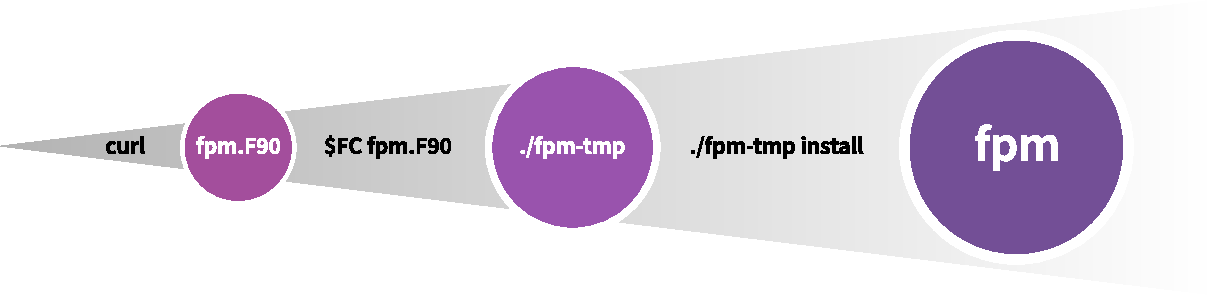
\includegraphics[width=.9\textwidth]{Figures/bootstrapping.pdf}
\end{frame}


\section{Feature overview}

\begin{frame}{Command-line features}
   \begin{columns}
      \hskip.1\textwidth
      \begin{column}{.6\textwidth}
         \begin{itemize}
            \item handles (sub)module interdependencies
            \item automatically finds executables and tests
         \end{itemize}
      \end{column}
   \end{columns}
   \vskip2ex

   \begin{columns}
      \begin{column}{.4\textwidth}
         \begin{itemize}
            \item runs executables and examples
            \item wildcard globbing for selection
         \end{itemize}
         \vskip5ex

         \begin{itemize}
            \item finds and runs test executables
            \item allows running tests in debugger
         \end{itemize}
      \end{column}
      \begin{column}{.3\textwidth}
         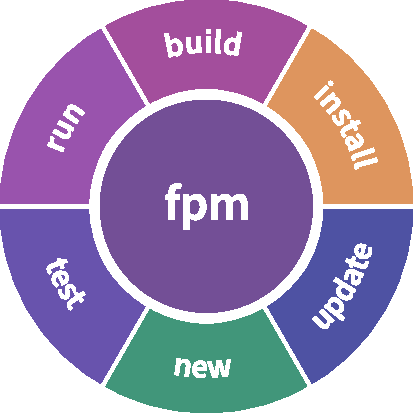
\includegraphics[width=\textwidth]{Figures/features.pdf}
      \end{column}
      \begin{column}{.4\textwidth}
         \begin{itemize}
            \item automatically installs project
            \item user prefix used by default
         \end{itemize}
         \vskip5ex

         \begin{itemize}
            \item updates all dependencies
            \item basic caching and locking
         \end{itemize}
      \end{column}
   \end{columns}
   \vskip1ex

   \begin{columns}
      \hskip.1\textwidth
      \begin{column}{.6\textwidth}
         \begin{itemize}
            \item creates new projects with fpm layout
            \item backfilling to update existing projects
         \end{itemize}
      \end{column}
   \end{columns}
\end{frame}

\begin{frame}{Layout of an fpm project}
   \begin{columns}
      \begin{column}{.6\textwidth}
         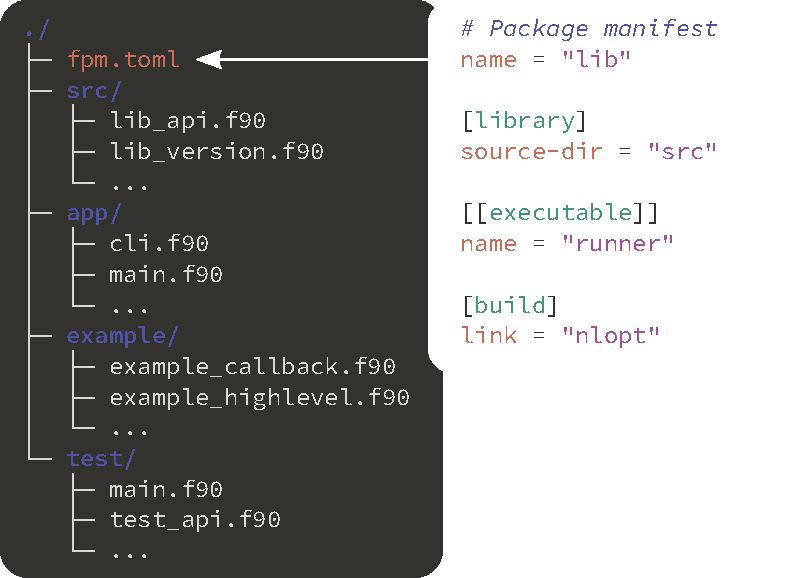
\includegraphics[width=\textwidth]{Figures/layout.pdf}
      \end{column}
      \hskip-1em
      \begin{column}{.45\textwidth}
         \begin{itemize}
            \item package manifest in \alert{TOML}
            \item limited complexity of build file
            \item mainly meta data of project\\
               (license, author, keywords, \ldots)
               \\[2ex]
            \item default layout requires only \alert{name}\\
               (\textcolor{blue}{src}, \textcolor{blue}{app}, \textcolor{blue}{example}, and \textcolor{blue}{test})
            \item \alert{source-dir} for customizing layout
               \\[2ex]
            \item executable names from \alert{program} unit
               \\[2ex]
            \item system libraries can be linked
               \\[2ex]
         \end{itemize}
      \end{column}
   \end{columns}
\end{frame}

\begin{frame}{First-class dependencies}
   \begin{itemize}
      \item dependencies are currently specified by referencing another project
         (\textit{e.\,g.} via git URL)
   \end{itemize}

   \begin{center}
      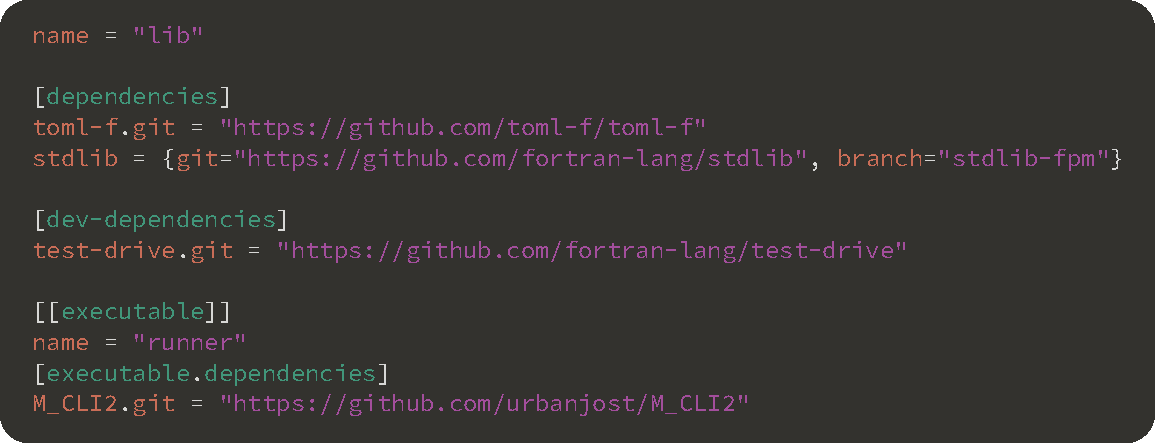
\includegraphics[width=.85\textwidth]{Figures/dependencies.pdf}
   \end{center}

   \begin{itemize}
      \item different scopes available beside full dependencies
      \item can depend on projects only for testing or limit dependencies to single executable
   \end{itemize}
\end{frame}

\begin{frame}{Extending fpm with plugins}
   \begin{itemize}
      \item package manifest provides space for third-party projects
      \item fpm is available as fpm package and can be used as dependency
      \item plugins are used automatically from the command-line
      \item useful for staging new features before integration in fpm
   \end{itemize}
   \vfill

   \begin{columns}
      \begin{column}{.45\textwidth}
         Searching for fpm packages: \alert{fpm-search}
         \begin{itemize}
            \item available from \textit{fpm search} command
            \item downloads the fpm registry
            \item search package names, descriptions
         \end{itemize}
      \end{column}
      \hskip1em
      \begin{column}{.45\textwidth}
         Documentation of intrinsics: \alert{fpm-man}
         \begin{itemize}
            \item available from \textit{fpm man} command
            \item access to documentation of intrinsics
            \item cross-platform, no man required
         \end{itemize}
      \end{column}
   \end{columns}
\end{frame}


\section{Summary and outlook}

\begin{frame}{Adoption of fpm}
   \begin{columns}
      \begin{column}{.5\textwidth}
         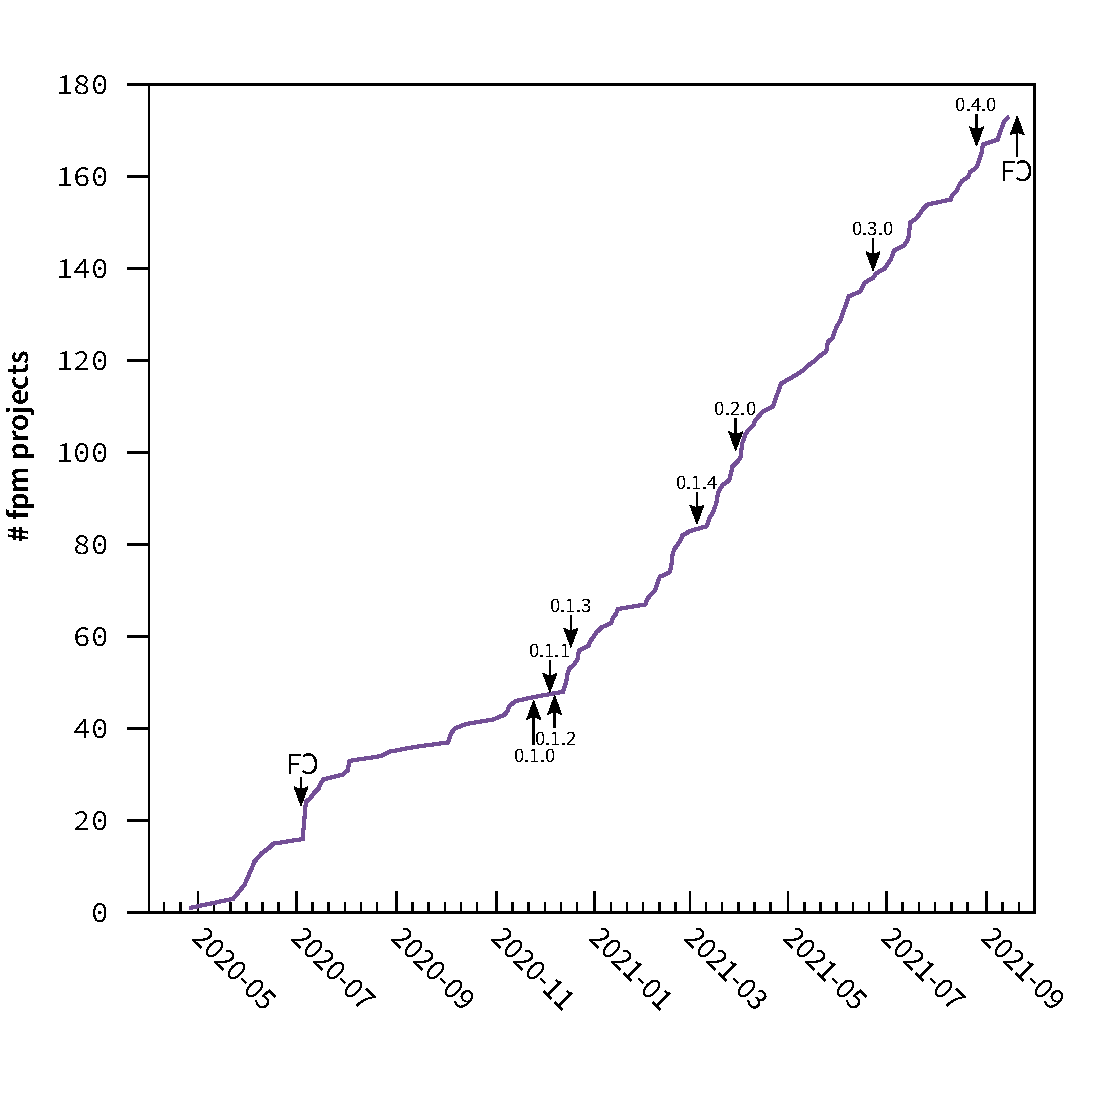
\includegraphics[width=\textwidth]{Figures/fpm-projects.pdf}
         \vskip-2ex

         \scriptsize
         Data collected from GitHub and GitLab on 15th Sep, 2021  % TODO: Update
      \end{column}
      \hskip-1em
      \begin{column}{.55\textwidth}
         \begin{itemize}
            \item today \alert{173} open source projects are using fpm  % TODO: Update
            \item ca. \alert{160} unique developers have contributed\\ to those projects  % TODO: Update
            \item \alert{62} contributors at the fpm project
            \item code contributions from \alert{21} developers to fpm
            \item hosted on GitHub (MIT licensed):\\\alert{https://github.com/fortran-lang/fpm}
         \end{itemize}
      \end{column}
   \end{columns}
\end{frame}

\begin{frame}{Open questions}
   \begin{itemize}
      \item can we integrate fpm seamlessly with other packaging ecosystems
   \end{itemize}
\end{frame}

\end{document}
